\begin{lstlisting}[language=Java]
  public static int binary2decimal(String string) {
1:  int decimalNumber = 0;                      
    int exponent = 0;
    char currentChar;
    CharacterIterator stringIterator = 
    new StringCharacterIterator(string);
    currentChar = stringIterator.last();

2:  while ((currentChar != CharacterIterator.DONE) 
    && (decimalNumber < Integer.MAX_VALUE)) {
3:    if (currentChar != '0' && currentChar != '1')
4:      return -1;

5:    if (currentChar == '1')
6:      decimalNumber += Math.pow(2, exponent);

7:    exponent++;
8:    currentChar = stringIterator.previous();
    }
9:  return decimalNumber;
  }
\end{lstlisting}
Es soll die 1 die ganzen Zuweisungen vor der while-loop umfassen. Der Kontrollflussgraph sieht wie folgt aus:
\begin{figure}[H]
  \centering
  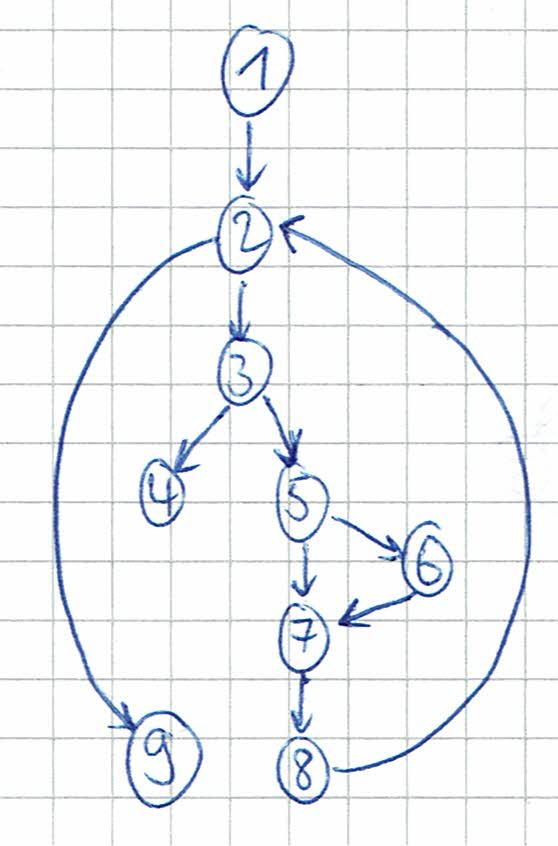
\includegraphics{2_cont.jpg}
\end{figure}
\noindent F\"ur die Anweisungsabdeckung reichen 2 F\"alle:
\begin{itemize}
    \item eine g\"ultige Eingabe, z.B. "3" (Ablauf: 1,2,3,4)
    \item eine g\"ultige Eingabe mit mindestens einer 1, zum Beispiel "1" (Ablauf: 1,2,3,5,6,7,8,2,9)
\end{itemize}
F\"ur die Zweigabdeckung gen\"ugen auch 2 F\"alle:
\begin{itemize}
    \item eine ung\"ultige Eingabe, z.B. "3" (Ablauf: 1,2,3,4)
    \item eine g\"ultige Eingabe mit Einsen und 0en, z.B. "10" (Ablauf: 1,2,3,5,6,7,8,2,3,5,7,8,2,9)
\end{itemize}
F\"ur die Pfadabdeckung gen\"ugen 10 F\"alle:
\begin{itemize}
    \item die Eingaben ''(leerer String),"2","02","12","00","01","10","11","0","1"
\end{itemize}